\RequirePackage{luatex85}
\documentclass{beamer}

\mode<presentation>
{
  \usetheme{metropolis}
  \usecolortheme{default}
  \usefonttheme{default}
  \setbeamertemplate{navigation symbols}{}
  \setbeamertemplate{caption}[numbered]
}


\usepackage[english]{babel}
\usepackage[utf8x]{inputenc}
\usepackage{xifthen} % If statements in tex are trash
\usepackage{tikz}    % Allows us to draw diagrams
\usepackage{gensymb} % Degree symbol

\usepackage{graphicx}
\graphicspath{{./img/claire/}}

%{{{ Bracelets
\directlua{dofile("bracelet.lua")}                                                % Import lua code
\newcommand{\bracelet}[2][]{
\ifthenelse{\isempty{#1}}{\directlua{bracelet(#2)}}{\directlua{bracelet(#2,#1)}}} % Bind latex to lua
%}}}
%{{{ Crosses
\newcommand{\cross}{
    	\draw[thick] (-1,3) -- ++(2,0)  --
        	      ++ (0,-2) -- ++(2,0)  --
                ++ (0,-2) -- ++(-2,0) --
                ++ (0,-2) -- ++(-2,0) --
                ++ (0,2)  -- ++(-2,0) --
                ++ (0,2)  -- ++(2,0)  -- ++(0,2);
}
\newcommand{\numberedcross}{
    	\draw[thick] (-1,3) -- node[fill=bg](1){1} ++(2,0)  -- node[fill=bg](2){2}
        	      ++ (0,-2) -- node[fill=bg](3){3} ++(2,0)  -- node[fill=bg](4){4}
                ++ (0,-2) -- node[fill=bg](5){5} ++(-2,0) -- node[fill=bg](6){6}
                ++ (0,-2) -- node[fill=bg](7){7} ++(-2,0) -- node[fill=bg](8){8}
                ++ (0,2)  -- node[fill=bg](9){9} ++(-2,0) -- node[fill=bg](10){10}
                ++ (0,2)  -- node[fill=bg](11){11} ++(2,0) -- node[fill=bg](12){12} ++(0,2);
}
%}}}
%{{{ Partial Ellipse
%Borrowed from SE
\tikzset{
	partial ellipse/.style args={#1:#2:#3}{
		insert path={+ (#1:#3) arc (#1:#2:#3)}
	}
}
%}}}
\title{Counting With Symmetries}
\author{Amber McKeough, Carlos Lira, Clarisse Bonnand, Ethan Kowalenko, Ethan Rooke, Reid Booth, Xavier Ramos}
\institute{UC Riverside}
\date{Thursday, June 1\textsuperscript{st}}

\begin{document}

\begin{frame}
  \titlepage
\end{frame}

%{{{ Introduction
\section{Introduction}
\begin{frame}{Introduction - Reid}
\begin{columns}[T]
\begin{column}{.48\textwidth}
	\begin{center}
    \begin{tikzpicture}
    	\draw (0,0) -- (5,0);
        \node[circle, fill=fg,inner sep=0pt,minimum size=.85cm] at (0,0) {};
        \node[circle, fill=bg,inner sep=0pt,minimum size=.82cm] at (0,0) {};
        \node[circle, fill=fg,inner sep=0pt,minimum size=.85cm] at (1,0) {};
        \node[circle, fill=bg,inner sep=0pt,minimum size=.82cm] at (1,0) {};
        \node[circle, fill=fg,inner sep=0pt,minimum size=.85cm] at (2,0) {};
        \node[circle, fill=bg,inner sep=0pt,minimum size=.82cm] at (2,0) {};
        \node[circle, fill=fg,inner sep=0pt,minimum size=.85cm] at (3,0) {};
        \node[circle, fill=bg,inner sep=0pt,minimum size=.82cm] at (3,0) {};
        \node[circle, fill=fg,inner sep=0pt,minimum size=.85cm] at (4,0) {};
        \node[circle, fill=bg,inner sep=0pt,minimum size=.82cm] at (4,0) {};
        \node[circle, fill=fg,inner sep=0pt,minimum size=.85cm] at (5,0) {};
        \node[circle, fill=bg,inner sep=0pt,minimum size=.82cm] at (5,0) {};
    \end{tikzpicture}
    \newline
	\begin{tikzpicture}[scale=0.5, transform shape]
    	\bracelet{"white white white white white white"}
    \end{tikzpicture}
    \end{center}
\end{column}%
\hfill%
\begin{column}{.48\textwidth}
	\begin{itemize}
		\item
        	We have black and white beads, and want to make
            a 6 bead bracelet.
        \item
        	Well, we have 6 beads and 2 choices per bead
            so $2^6$ right?
        \item
        	This is only true so long as you don't care about symmetry.
	\end{itemize}
\end{column}%
\end{columns}
\end{frame}

\begin{frame}{Symmetry?}
	\begin{center}
	\begin{tikzpicture}[scale=0.5, transform shape]
    	\bracelet{"white black black black black black"}
        \begin{scope}[shift={(9cm,0)}]
        \bracelet{"black black black white black black"}
        \end{scope}
    \end{tikzpicture}
    \end{center}
    \begin{itemize}
    \item
    	Our initial count considers these different
    \item
    	But one is just the other one rotated
    \item
    	We would like to consider these as the same when we count
    \end{itemize}
\end{frame}

\begin{frame}{The hard way}
	We can count this way by making a table of bracelets and counting how many different bracelets
    can be made via rotations of that bracelet.
\end{frame}

\begin{frame}{The hard way}
	Specifically, we want to count colorings with rotations by picking combinations of beads and treating them as equal when they're rotations of each other:
	\begin{center}
    \raisebox{-.45\height}{\begin{tikzpicture}[scale=0.30, transform shape]
    	\bracelet{"white black black black black black"}
    \end{tikzpicture}} =
    \raisebox{-.45\height}{\begin{tikzpicture}[scale=0.30, transform shape]
        \begin{scope}[shift={(9,0)}]
        	\bracelet{"black white black black black black"}
        \end{scope}
    \end{tikzpicture}} =
    \raisebox{-.45\height}{\begin{tikzpicture}[scale=0.30, transform shape]
        \begin{scope}[shift={(18,0)}]
        	\bracelet{"black black white black black black"}
        \end{scope}
    \end{tikzpicture}} =\newline
    \raisebox{-.45\height}{\begin{tikzpicture}[scale=0.30, transform shape]
        \bracelet{"black black black white black black"}
    \end{tikzpicture}} =
    \raisebox{-.45\height}{\begin{tikzpicture}[scale=0.30, transform shape]
        \begin{scope}[shift={(9,0)}]
        	\bracelet{"black black black black white black"}
        \end{scope}
    \end{tikzpicture}} =
    \raisebox{-.45\height}{\begin{tikzpicture}[scale=0.30, transform shape]
        \begin{scope}[shift={(18,0)}]
        	\bracelet{"black black black black black white"}
        \end{scope}
    \end{tikzpicture}}
    \end{center}
\end{frame}

\begin{frame}{The hard way}
    \begin{columns}[T]
    \begin{column}{0.48\textwidth}
    \begin{tabular}{r l}
    	\raisebox{-.45\height}{\begin{tikzpicture}[scale=0.25, transform shape]
    		\bracelet{"white white white white white white"}
        	\begin{scope}[shift={(9,0)}]
        		\bracelet{"black black black black black black"}
        	\end{scope}
    	\end{tikzpicture}} & 2\to2 \\
        \pause
        \raisebox{-.45\height}{\begin{tikzpicture}[scale=0.25, transform shape]
    		\bracelet{"black white white white white white"}
        	\begin{scope}[shift={(9,0)}]
        		\bracelet{"white black black black black black"}
        	\end{scope}
    	\end{tikzpicture}} & 12\to2 \\
        \pause
        \raisebox{-.45\height}{\begin{tikzpicture}[scale=0.25, transform shape]
    		\bracelet{"black black white white white white"}
        	\begin{scope}[shift={(9,0)}]
        		\bracelet{"white white black black black black"}
        	\end{scope}
    	\end{tikzpicture}} & 12\to2 \\

        \raisebox{-.45\height}{\begin{tikzpicture}[scale=0.25, transform shape]
    		\bracelet{"black white black white white white"}
        	\begin{scope}[shift={(9,0)}]
        		\bracelet{"white black white black black black"}
        	\end{scope}
    	\end{tikzpicture}} & 12\to2
    \end{tabular}
    \end{column}%
	\hfill%
	\begin{column}{.48\textwidth}
        \begin{tabular}{r l}
    	\raisebox{-.45\height}{\begin{tikzpicture}[scale=0.25, transform shape]
    		\bracelet{"black white white black white white"}
        	\begin{scope}[shift={(9cm,0)}]
        		\bracelet{"white black black white black black"}
        	\end{scope}
    	\end{tikzpicture}} & 6\to2 \\

        \raisebox{-.45\height}{\begin{tikzpicture}[scale=0.25, transform shape]
    		\bracelet{"black black white black white white"}
        	\begin{scope}[shift={(9cm,0)}]
        		\bracelet{"white white black white black black"}
        	\end{scope}
    	\end{tikzpicture}} & 12\to2 \\

        \raisebox{-.45\height}{\begin{tikzpicture}[scale=0.25, transform shape]
    		\bracelet{"black black black white white white"}
    	\end{tikzpicture}} & 6\to1 \\

        \raisebox{-.45\height}{\begin{tikzpicture}[scale=0.25, transform shape]
    		\bracelet{"black white black white black white"}
    	\end{tikzpicture}} & 2\to1

        \end{tabular}
    \end{column}
    \end{columns}
\end{frame}

\begin{frame}{Flips and Colorings}
	\begin{columns}[T]
    \begin{column}{0.48\textwidth}
	\begin{itemize}
    	\item However, the count is different if we allow for more actions than just rotations.
        \item Another action we could add is flipping the bracelet over.
        \item This results in different unique colorings.
	\end{itemize}
    \end{column}
    \begin{column}{0.48\textwidth}
    	\raisebox{-.45\height}{\begin{tikzpicture}[scale=0.25, transform shape]
    		\bracelet{"black black white black white white"}
        \end{tikzpicture}} $\neq$
    	\raisebox{-.45\height}{\begin{tikzpicture}[scale=0.25, transform shape]
    		\bracelet{"black white white black white black"}
        \end{tikzpicture}}
        \newline when no flips are allowed.\newline
        \raisebox{-.45\height}{\begin{tikzpicture}[scale=0.25, transform shape]
    		\bracelet{"black black white black white white"}
        \end{tikzpicture}} =
    	\raisebox{-.45\height}{\begin{tikzpicture}[scale=0.25, transform shape]
    		\bracelet{"black white white black white black"}
        \end{tikzpicture}}
        \newline when flips are allowed.\newline
    \end{column}
    \end{columns}
\end{frame}

\begin{frame}{Dihedral Group and Group Actions}
	\begin{itemize}
    	\item We seek to generalize the types of things we can do to sets with the right symmetries.
        \item To get an idea of these, we will look at the symmetries of an equilateral triangle.
		\item We will let $\Delta$ denote the set of points that make up an equilateral triangle.
		\item We want to describe the symmetries of this triangle.
		\item We then want to think about the actions that make up these symmetries more generally.
	\end{itemize}
\end{frame}

\begin{frame}{Dihedral Group and Group Actions}
\begin{center}
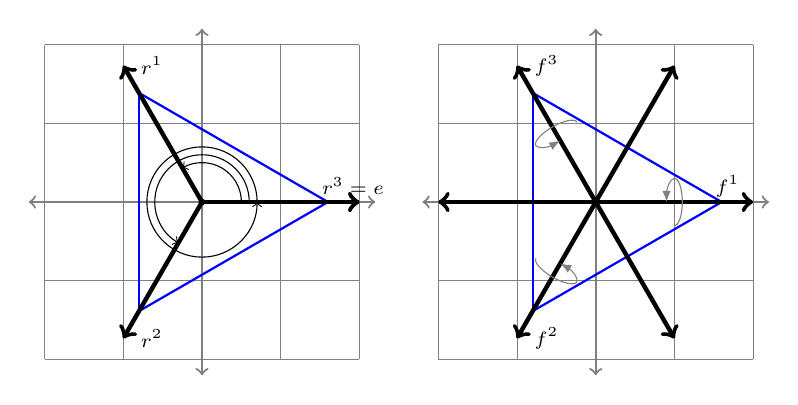
\begin{tikzpicture}
\tikzstyle{every node}=[font=\scriptsize]
% Draw background grid and axes
\draw[step=1cm,gray,very thin] (-2,-2) grid (2,2);
\draw[step=1cm,gray,very thin] (-7,-2) grid (-3,2);

\draw[gray, thick, <->] (-2.2-5,0) -- (2.2-5,0); %left axes, just shifted
\draw[gray, thick, <->] (0-5,-2.2) -- (0-5,2.2);
\filldraw[black] (0-5,0) circle (1pt) node[anchor=west] {};

\draw[gray, thick, <->] (-2.2,0) -- (2.2,0); % right axes
\draw[gray, thick, <->] (0,-2.2) -- (0,2.2);
\filldraw[black] (0,0) circle (1pt) node[anchor=west] {};

% Draw triangle
\draw[blue, thick] (-1*4/5-5,1.732*4/5) -- (-1*4/5-5,-1.732*4/5);
\draw[blue, thick] (2*4/5-5,0) -- (-1*4/5-5,-1.732*4/5);
\draw[blue, thick] (-1*4/5-5,1.732*4/5) -- (2*4/5-5,0);
\draw[blue, thick] (-1*4/5,1.732*4/5) -- (-1*4/5,-1.732*4/5);
\draw[blue, thick] (2*4/5,0) -- (-1*4/5,-1.732*4/5);
\draw[blue, thick] (-1*4/5,1.732*4/5) -- (2*4/5,0);


% -----------------------------------------------------
\pause
\draw[->] (0.5-5,0) arc (0:120:0.5cm);
\draw[ultra thick, black,->] (0-5,0) -- (2-5,0);
\draw[ultra thick, black,->] (0-5,0) -- (-1-5,1.732);
\filldraw[black] (-0.9-5,1.732) circle (0pt) node[anchor=west] {$r^1$};
\pause
\draw[->] (0.6-5,0) arc (0:240:0.6cm);
\draw[ultra thick, black,->] (0-5,0) -- (-1-5,-1.732);
\filldraw[black] (-0.9-5,-1.732) circle (0pt) node[anchor=west] {$r^2$};
\pause
\draw[->] (0.7-5,0) arc (0:360:0.7cm);
\draw[ultra thick, black,->] (0-5,0) -- (2-5,0);
\filldraw[black] (1.4-5,0.2) circle (0pt) node[anchor=west] {$r^3=e$};
\pause
% -----------------------------------------------------
\draw[ultra thick, black,<->] (-2,0) -- (2,0);
\filldraw[black] (1.4,0.2) circle (0pt) node[anchor=west] {$f^1$};
\draw[rotate=270, gray, thin, -latex] (0,1) [partial ellipse=0:270:0.3cm and 0.1cm];
\pause
\draw[ultra thick, black,<->] (1,1.732) -- (-1,-1.732);
\filldraw[black] (-0.9,-1.732) circle (0pt) node[anchor=west] {$f^2$};
\draw[rotate=150, gray, thin, -latex] (0,1) [partial ellipse=0:270:0.3cm and 0.1cm];
\pause
\draw[ultra thick, black,<->] (1,-1.732) -- (-1,1.732);
\filldraw[black] (-0.9,1.732) circle (0pt) node[anchor=west] {$f^3$};
\draw[rotate=30, gray, thin, -latex] (0,1) [partial ellipse=0:270:0.3cm and 0.1cm];




\end{tikzpicture}

\end{center}
\end{frame}
\begin{frame}{Dihedral Group and Group Actions}
	\begin{center}
		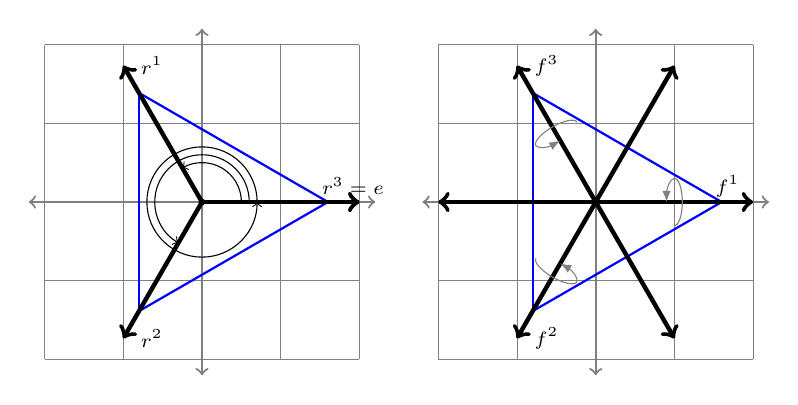
\begin{tikzpicture}
		\tikzstyle{every node}=[font=\scriptsize]
		% Draw background grid and axes
		\draw[step=1cm,gray,very thin] (-2,-2) grid (2,2);
		\draw[step=1cm,gray,very thin] (-7,-2) grid (-3,2);

		\draw[gray, thick, <->] (-2.2-5,0) -- (2.2-5,0); %left axes, just shifted
		\draw[gray, thick, <->] (0-5,-2.2) -- (0-5,2.2);
		\filldraw[black] (0-5,0) circle (1pt) node[anchor=west] {};

		\draw[gray, thick, <->] (-2.2,0) -- (2.2,0); % right axes
		\draw[gray, thick, <->] (0,-2.2) -- (0,2.2);
		\filldraw[black] (0,0) circle (1pt) node[anchor=west] {};

		% Draw triangle
		\draw[blue, thick] (-1*4/5-5,1.732*4/5) -- (-1*4/5-5,-1.732*4/5);
		\draw[blue, thick] (2*4/5-5,0) -- (-1*4/5-5,-1.732*4/5);
		\draw[blue, thick] (-1*4/5-5,1.732*4/5) -- (2*4/5-5,0);
		\draw[blue, thick] (-1*4/5,1.732*4/5) -- (-1*4/5,-1.732*4/5);
		\draw[blue, thick] (2*4/5,0) -- (-1*4/5,-1.732*4/5);
		\draw[blue, thick] (-1*4/5,1.732*4/5) -- (2*4/5,0);


		% -----------------------------------------------------

		\draw[->] (0.5-5,0) arc (0:120:0.5cm);
		\draw[ultra thick, black,->] (0-5,0) -- (2-5,0);
		\draw[ultra thick, black,->] (0-5,0) -- (-1-5,1.732);
		\filldraw[black] (-0.9-5,1.732) circle (0pt) node[anchor=west] {$r^1$};

		\draw[->] (0.6-5,0) arc (0:240:0.6cm);
		\draw[ultra thick, black,->] (0-5,0) -- (-1-5,-1.732);
		\filldraw[black] (-0.9-5,-1.732) circle (0pt) node[anchor=west] {$r^2$};

		\draw[->] (0.7-5,0) arc (0:360:0.7cm);
		\draw[ultra thick, black,->] (0-5,0) -- (2-5,0);
		\filldraw[black] (1.4-5,0.2) circle (0pt) node[anchor=west] {$r^3=e$};

		% -----------------------------------------------------
		\draw[ultra thick, black,<->] (-2,0) -- (2,0);
		\filldraw[black] (1.4,0.2) circle (0pt) node[anchor=west] {$f^1$};
		\draw[rotate=270, gray, thin, -latex] (0,1) [partial ellipse=0:270:0.3cm and 0.1cm];

		\draw[ultra thick, black,<->] (1,1.732) -- (-1,-1.732);
		\filldraw[black] (-0.9,-1.732) circle (0pt) node[anchor=west] {$f^2$};
		\draw[rotate=150, gray, thin, -latex] (0,1) [partial ellipse=0:270:0.3cm and 0.1cm];

		\draw[ultra thick, black,<->] (1,-1.732) -- (-1,1.732);
		\filldraw[black] (-0.9,1.732) circle (0pt) node[anchor=west] {$f^3$};
		\draw[rotate=30, gray, thin, -latex] (0,1) [partial ellipse=0:270:0.3cm and 0.1cm];




		\end{tikzpicture}

	\end{center}
	$D_3=\{e,r^1,r^2,f^1,f^2,f^3\}$ is the dihedral group on $3$ elements.

	We say $D_3$ acts on $\Delta$, or $D_3\circlearrowright\Delta$.
\end{frame}

\begin{frame}{$D_4$}
	\begin{center}
		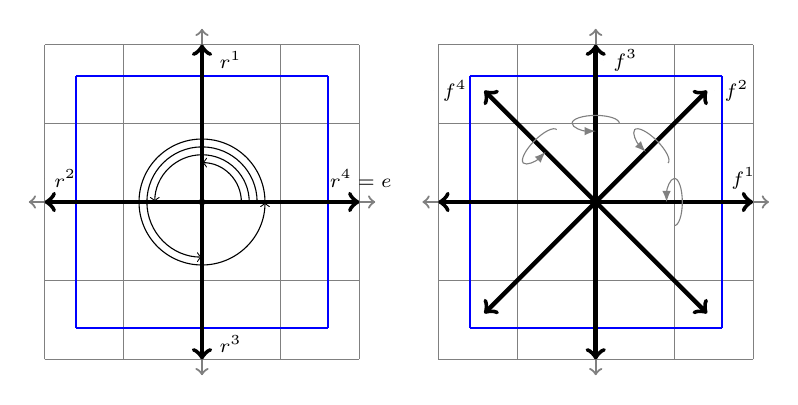
\begin{tikzpicture}
		\tikzstyle{every node}=[font=\scriptsize]
		% Draw background grid and axes
		\draw[step=1cm,gray,very thin] (-2,-2) grid (2,2);
		\draw[step=1cm,gray,very thin] (-7,-2) grid (-3,2);

		\draw[gray, thick, <->] (-2.2-5,0) -- (2.2-5,0); %left axes, just shifted
		\draw[gray, thick, <->] (0-5,-2.2) -- (0-5,2.2);
		\filldraw[black] (0-5,0) circle (1pt) node[anchor=west] {};

		\draw[gray, thick, <->] (-2.2,0) -- (2.2,0); % right axes
		\draw[gray, thick, <->] (0,-2.2) -- (0,2.2);
		\filldraw[black] (0,0) circle (1pt) node[anchor=west] {};

		% Draw triangle
		\draw[blue, thick] (-2*4/5-5,2*4/5) -- (-2*4/5-5,-2*4/5);
		\draw[blue, thick] (2*4/5-5,-2*4/5) -- (-2*4/5-5,-2*4/5);
		\draw[blue, thick] (-2*4/5-5,2*4/5) -- (2*4/5-5,2*4/5);
		\draw[blue, thick] (2*4/5-5,-2*4/5) -- (2*4/5-5,2*4/5);
		\draw[blue, thick] (-2*4/5,2*4/5) -- (-2*4/5,-2*4/5);
		\draw[blue, thick] (2*4/5,-2*4/5) -- (-2*4/5,-2*4/5);
		\draw[blue, thick] (-2*4/5,2*4/5) -- (2*4/5,2*4/5);
		\draw[blue, thick] (2*4/5,-2*4/5) -- (2*4/5,2*4/5);


		% -----------------------------------------------------

		\draw[->] (0.5-5,0) arc (0:90:0.5cm);
		\draw[ultra thick, black,->] (0-5,0) -- (-5,2);
		\filldraw[black] (0.1-5,1.8) circle (0pt) node[anchor=west] {$r^1$};

		\draw[->] (0.6-5,0) arc (0:180:0.6cm);
		\draw[ultra thick, black,->] (0-5,0) -- (-2-5,0);
		\filldraw[black] (-2-5,0.3) circle (0pt) node[anchor=west] {$r^2$};

		\draw[->] (0.7-5,0) arc (0:270:0.7cm);
		\draw[ultra thick, black,->] (0-5,0) -- (-5,-2);
		\filldraw[black] (0.1-5,-1.8) circle (0pt) node[anchor=west] {$r^3$};

		\draw[->] (0.8-5,0) arc (0:360:0.8cm);
		\draw[ultra thick, black,->] (0-5,0) -- (2-5,0);
		\filldraw[black] (1.5-5,0.3) circle (0pt) node[anchor=west] {$r^4=e$};

		% -----------------------------------------------------
		\draw[ultra thick, black,<->] (-2,0) -- (2,0);
		\filldraw[black] (1.6,0.3) circle (0pt) node[anchor=west] {$f^1$};
		\draw[rotate=270, gray, thin, -latex] (0,1) [partial ellipse=0:270:0.3cm and 0.1cm];

		\draw[ultra thick, black,<->] (-1.414,-1.414) -- (1.414,1.414);
		\filldraw[black] (1.414+0.1,1.414) circle (0pt) node[anchor=west] {$f^2$};
		\draw[rotate=315, gray, thin, -latex] (0,1) [partial ellipse=0:270:0.3cm and 0.1cm];

		\draw[ultra thick, black,<->] (0,-2) -- (0,2);
		\filldraw[black] (0.1,1.8) circle (0pt) node[anchor=west] {$f^3$};
		\draw[rotate=0, gray, thin, -latex] (0,1) [partial ellipse=0:270:0.3cm and 0.1cm];

		\draw[ultra thick, black,<->] (-1.414,1.414) -- (1.414,-1.414);
		\filldraw[black] (-1.414-0.65,1.414) circle (0pt) node[anchor=west] {$f^4$};
		\draw[rotate=45, gray, thin, -latex] (0,1) [partial ellipse=0:270:0.3cm and 0.1cm];




		\end{tikzpicture}

	\end{center}
	$D_4=\{e,r^1,r^2,r^3,f^1,f^2,f^3,f^4\}$ is the dihedral group on $4$ elements.

	This generalizes to $D_n$, the dihedral group on $n$ elements: it's a group of $2n$ elements with $n$ rotations and $n$ flips.
\end{frame}

\begin{frame}{The Goal}

    The goal of this talk is to develop a framework for
    answering coloring questions like these where symmetry
    is crucial
\end{frame}

%}}}
%{{{ Polya Build Up
\section{Polya Build up - Ethan}

\begin{frame}{Permutations}
	\begin{itemize}
	\item A permutation is a bijection from a set S into itself
    \item Can be viewed as changing the order of elements
    \item Consider the set $S = \{1,2,3,4\}$ And let $f : S \to S$ be defined
    \begin{align*}
    	f(1) &= 2 \\
        f(2) &= 1 \\
        f(3) &= 4 \\
        f(4) &= 3 \\
    \end{align*}
	\end{itemize}
\end{frame}

\begin{frame}{Permutations}
  To specify permutations we use cycle notation.
  \begin{center}
    \begin{tikzpicture}
      \draw[draw=bg] (-.5,.5) -- (2.5,.5) --
                     (2.5,-4.5) -- (-.5,-4.5);

      \node<2-> at (0,0) (1) {1};
      \node<2-> at (0,-1) (2) {2};
      \node<2-> at (0,-2) (3) {3};
      \node<2-> at (0,-3) (4) {4};

      \node<2-> at (2,0) (1') {1};
      \node<2-> at (2,-1) (2') {2};
      \node<2-> at (2,-2) (3') {3};
      \node<2-> at (2,-3) (4') {4};
      %{{{ (12)(34)
      \draw<2>[thick, ->] (1) to (2');
      \draw<2>[thick, ->] (2) to (1');
      \draw<2>[thick, ->] (3) to (4');
      \draw<2>[thick, ->] (4) to (3');
      \node<2> at (1,-4) {$(12)(34)$};
      %}}}
      %{{{ (123)(4)
      \draw<4-7>[thick, ->] (1) to (2');
      \draw<5-7>[thick, ->] (2) to (3');
      \draw<6-7>[thick, ->] (3) to (1');
      \draw<7>[thick, ->] (4) to (4');
      \node<3-7> at (1,-4) {$(123)(4)$};
      %}}}
      %{{{ Identity example
      \draw<8>[thick, ->] (1) to (1');
      \draw<8>[thick, ->] (2) to (2');
      \draw<8>[thick, ->] (3) to (3');
      \draw<8>[thick, ->] (4) to (4');
      \node<8> at (1,-4) {$(1)(2)(3)(4)=e$};
      %}}}
    \end{tikzpicture}
  \end{center}
\end{frame}

\begin{frame}{Colorings}
  A coloring $c$ is a map from our set of objects into
  our set of colors.
  \begin{center}
    \begin{tikzpicture}
      \draw[draw=bg] (-.5,.5) -- (2.5,.5) --
                     (2.5,-4.5) -- (-.5,-4.5);

      \node<2-> at (0,0) (1) {1};
      \node<2-> at (0,-1) (2) {2};
      \node<2-> at (0,-2) (3) {3};
      \node<2-> at (0,-3) (4) {4};

      \node<2-> at (2,-1) (b) {b};
      \node<2-> at (2,-2) (w) {w};

      %{{{ Coloring 1
      \draw<2>[thick,->] (1) to (b);
      \draw<2>[thick,->] (2) to (w);
      \draw<2>[thick,->] (3) to (b);
      \draw<2>[thick,->] (4) to (w);
      \node<2> at (1,-4) {$(bwbw)$};
      %}}}
      %{{{ Coloring 2
      \draw<3>[thick,->] (1) to (w.west);
      \draw<3>[thick,->] (2) to (w.west);
      \draw<3>[thick,->] (3) to (b.west);
      \draw<3>[thick,->] (4) to (b.west);
      \node<3> at (1,-4) {$(wwbb)$};
      %}}}
    \end{tikzpicture}
  \end{center}
\end{frame}

\begin{frame}{Permuting Colorings}
  As a coloring is a map from our set of objects to
  our set of colors, if we compose a coloring $c$
  with a permutation we get a new coloring.
  \begin{center}
    \begin{tikzpicture}
      \draw[draw=bg] (-.5,.5) -- (4.5,.5) --
                     (4.5,-4.5) -- (-.5,-4.5);

      \node<2-> at (0,0) (1) {1};
      \node<2-> at (0,-1) (2) {2};
      \node<2-> at (0,-2) (3) {3};
      \node<2-> at (0,-3) (4) {4};

      \node<2-> at (2,0) (1') {1};
      \node<2-> at (2,-1) (2') {2};
      \node<2-> at (2,-2) (3') {3};
      \node<2-> at (2,-3) (4') {4};

      \node<2-> at (4,-1) (b) {b};
      \node<2-> at (4,-2) (w) {w};

      \node<3-> at (6,0) (1'') {1};
      \node<3-> at (6,-1) (2'') {2};
      \node<3-> at (6,-2) (3'') {3};
      \node<3-> at (6,-3) (4'') {4};

      \node<3-> at (8,-1) (b') {b};
      \node<3-> at (8,-2) (w') {w};

      %{{{ (12)(34)
      \draw<2->[thick, ->] (1) to (2');
      \draw<2->[thick, ->] (2) to (1');
      \draw<2->[thick, ->] (3) to (4');
      \draw<2->[thick, ->] (4) to (3');
      \node<2-> at (1,-4) {$(12)(34)$};
      \node<2-> at (2,-4) {$\circ$};
      %}}}

      %{{{ Coloring 1
      \draw<2->[thick,->] (1') to (b);
      \draw<2->[thick,->] (2') to (w);
      \draw<2->[thick,->] (3') to (b);
      \draw<2->[thick,->] (4') to (w);
      \node<2-> at (3,-4) {$(bwbw)$};
      %}}}

      %{{{ Coloring 2
      \draw<4->[thick,->] (1'') to (w');
      \draw<5->[thick,->] (2'') to (b');
      \draw<6->[thick,->] (3'') to (w');
      \draw<7->[thick,->] (4'') to (b');
      \node<8-> at (7,-4) {$(wbwb)$};
      %}}}
    \end{tikzpicture}
  \end{center}
\end{frame}

\begin{frame}{Symmetry}
	This gives us a language to discuss symmetry now. Consider the two bracelets from earlier:
	\begin{center}
    	\begin{tikzpicture}[scale=0.5, transform shape]
    		\bracelet[true]{"white black black black black black"}
        	\uncover<2>{
            \draw[|->, thick] (3.75,0) -- (8.25,0);
        	\node[above] at (6,0.1) {\huge (14)(25)(36)};}
        	\begin{scope}[shift={(12,0)}]
        	\bracelet[true]{"black black black white black black"}
        	\end{scope}
    	\end{tikzpicture}
    \end{center}
\end{frame}

\begin{frame}{Symmetry}
	Thus we can describe the symmetry of an object by defining the group of permutations we allow on it.

  Taking our bracelet example from earlier we see that our set of permutations is:
  \[\{e,(123456),(135)(246),(14)(25)(36),(153)(264),(165432)\}\]
\end{frame}
%}}}
%{{{ How to use polya
\section{Abstracting Polya from the cycle index}

\begin{frame}
\begin{itemize}

\item We can use the six bead example and definition of permutations to generalize properties from equations and definitions.

\item Definition: Let G be a group whose elements are the permutations on S and ${|S|} = m$. Next we let m variables $x_{1}, x_{2},...,x_{m}$ with nonnegative coefficients form the product $\beta = x_{1}^{\alpha_{1}}, x_{2}^{\alpha_{2}},...,x_{m}^{\alpha_{m}}$ for every permutation in G.

\item Also let $\alpha_{i}$ represents the the number of disjoint cycles of length $i$ in the given permutation.

\end{itemize}
\end{frame}

%%%

\begin{frame}
\begin{itemize}

\item We can obtain the cyle index of G $P_{G}(x_{1},x_{2},...,x_{m})=\frac{1}{\vert{G}\vert}\sum_{{\pi} \in G}x_{1}^{\alpha_{1}},x_{2}^{\alpha_{2}},...,x_{m}^{\alpha_{m}}$.

%\item Before we generalize further, lets describe some properties of the cycle index.

\end{itemize}
\end{frame}

%%%

\begin{frame}
\begin{itemize}
%under symmetries of rotation and reflection
\item For example, referring back to the 6 beaded example, we get the cycle index $P_{D_{6}}(x_{1},x_{2},x_{3},x_{4},x_{5},x_{6})=\frac{1}{9}(x_{1}^{6} + x_{6}^{1} + x_{3}^{2} + x_{2}^{3} + x_{3}^{2} + x_{6}^{1} + x_{2}^{2}x_{1}^{2} + x_{2}^{2}x_{1}^{2} + x_{2}^{2}x_{1}^{2})$.

\item Every term represent a permutation and the superscript represents the number of disjoint cycles in the permutation while the superscript represents the length of each cycle.

\item $7th$ term in the polynomial represents the permutation ${\pi} = (1)(26)(35)(4)$. Therefore two cycles of length two and two cycles of length one correspond to $x = x_{2}^{2}x_{1}^{2}$.


\end{itemize}
\end{frame}

%%%

\begin{frame}
\begin{itemize}

\item The purpose of the cycle index is to determine the number of distinct colorings acted on by the group of symmetries G.

\item For example, Let m equal the number of any distinct colors, we obtain the polynomial, $P_{D_{6}}(m,m,m,m)=\frac{1}{9}(m_{1}^{6} + 2m_{6}^{1} + 2m_{3}^{2} + m_{2}^{3} + 3m_{2}^{2}m_{1}^{2})$.

\item Specifically, when $m=2$ we obtain $P_{D_{6}}(2,2,2,2)=$.

\end{itemize}
\end{frame}

%%%% need to include slide of equivalent colorings

%%%

\begin{frame}
\begin{itemize}

\item While the cycle index tells us the number of distinct objects we seek, we can abstract even further to obtain not only the number of distinct objects but also an idea of the appearance of what each object should look like.

\item Polya's Enumeration Formula: Let S be a set of elements and G a group of permutations on S, where each permutation induces an equivalence relation on the colorings of S. The inventory of nonequivalent colorings of S using colors $c_{1},c_{2},...,c_{m}$ is the function $P_{G}(\sum_{j=1}^{m}c_{j},\sum_{j=1}^{m}c_{j}^{2},...,\sum_{j=1}^{m}c_{j}^{k})$.

\item As an observation, the k in $P_{G}(\sum_{j=1}^{m}c_{j},\sum_{j=1}^{m}c_{j}^{2},...,\sum_{j=1}^{m}c_{j}^{k})$ refers to the largest cycle length.


\end{itemize}
\end{frame}

%% To clarify how to use polya, and properties
%% observing properties from the polya's theorem and resorting back to necklace problem.

\begin{frame}
\begin{itemize}

\item Resorting back to our bead example, if we let b and w represent our two colors, then we obtain $P_{D_{4}}((b+w), (b^2+w^2), (b^3+w^3), (b^4+w^4)) = b^6 + b^5w + 3b^4w^2 + 4b^3w^3 + 3b^2w^4 + bw^5 + w^6$.

\item The coefficient, of each term, $A_{i}b^{k}w^{j}$ determines the number of possible distinct colorings on the six beaded bracelet using the colors b and w, i and j times for each bead.

\item for example, the third term $3b^4w^2$ corresponds to 3 possible colorings, coloring 4 bead's black and 2 bead's white.

\end{itemize}
\end{frame}
%}}}
%{{{ Ambers section
\section{Abstracting Polya from the cycle index}

\begin{frame}
\begin{itemize}

\item We can use the six bead example and definition of permutations to generalize properties from equations and definitions.

\item Definition: Let G be a group whose elements are the permutations on S and ${|S|} = m$. Next we let m variables $x_{1}, x_{2},...,x_{m}$ with nonnegative coefficients form the product $\beta = x_{1}^{\alpha_{1}}, x_{2}^{\alpha_{2}},...,x_{m}^{\alpha_{m}}$ for every permutation in G.

\item Also let $\alpha_{i}$ represents the the number of disjoint cycles of length $i$ in the given permutation.

\end{itemize}
\end{frame}

%%%

\begin{frame}
\begin{itemize}

\item We can obtain the cyle index of G $P_{G}(x_{1},x_{2},...,x_{m})=\frac{1}{\vert{G}\vert}\sum_{{\pi} \in G}x_{1}^{\alpha_{1}},x_{2}^{\alpha_{2}},...,x_{m}^{\alpha_{m}}$.

%\item Before we generalize further, lets describe some properties of the cycle index.

\end{itemize}
\end{frame}

%%%

\begin{frame}
\begin{itemize}
%under symmetries of rotation and reflection
\item For example, referring back to the 6 beaded example, we get the cycle index $P_{D_{6}}(x_{1},x_{2},x_{3},x_{4},x_{5},x_{6})=\frac{1}{9}(x_{1}^{6} + x_{6}^{1} + x_{3}^{2} + x_{2}^{3} + x_{3}^{2} + x_{6}^{1} + x_{2}^{2}x_{1}^{2} + x_{2}^{2}x_{1}^{2} + x_{2}^{2}x_{1}^{2})$.

\item Every term represent a permutation and the superscript represents the number of disjoint cycles in the permutation while the superscript represents the length of each cycle.

\item $7th$ term in the polynomial represents the permutation ${\pi} = (1)(26)(35)(4)$. Therefore two cycles of length two and two cycles of length one correspond to $x = x_{2}^{2}x_{1}^{2}$.


\end{itemize}
\end{frame}

%%%

\begin{frame}
\begin{itemize}

\item The purpose of the cycle index is to determine the number of distinct colorings acted on by the group of symmetries G.

\item For example, Let m equal the number of any distinct colors, we obtain the polynomial, $P_{D_{6}}(m,m,m,m)=\frac{1}{9}(m_{1}^{6} + 2m_{6}^{1} + 2m_{3}^{2} + m_{2}^{3} + 3m_{2}^{2}m_{1}^{2})$.

\item Specifically, when $m=2$ we obtain $P_{D_{6}}(2,2,2,2)=$.

\end{itemize}
\end{frame}

%%%% need to include slide of equivalent colorings

%%%

\begin{frame}
\begin{itemize}

\item While the cycle index tells us the number of distinct objects we seek, we can abstract even further to obtain not only the number of distinct objects but also an idea of the appearance of what each object should look like.

\item Polya's Enumeration Formula: Let S be a set of elements and G a group of permutations on S, where each permutation induces an equivalence relation on the colorings of S. The inventory of nonequivalent colorings of S using colors $c_{1},c_{2},...,c_{m}$ is the function $P_{G}(\sum_{j=1}^{m}c_{j},\sum_{j=1}^{m}c_{j}^{2},...,\sum_{j=1}^{m}c_{j}^{k})$.

\item As an observation, the k in $P_{G}(\sum_{j=1}^{m}c_{j},\sum_{j=1}^{m}c_{j}^{2},...,\sum_{j=1}^{m}c_{j}^{k})$ refers to the largest cycle length.


\end{itemize}
\end{frame}

%% To clarify how to use polya, and properties
%% observing properties from the polya's theorem and resorting back to necklace problem.

\begin{frame}
\begin{itemize}

\item Resorting back to our bead example, if we let b and w represent our two colors, then we obtain $P_{D_{4}}((b+w), (b^2+w^2), (b^3+w^3), (b^4+w^4)) = b^6 + b^5w + 3b^4w^2 + 4b^3w^3 + 3b^2w^4 + bw^5 + w^6$.

\item The coefficient, of each term, $A_{i}b^{k}w^{j}$ determines the number of possible distinct colorings on the six beaded bracelet using the colors b and w, i and j times for each bead.

\item for example, the third term $3b^4w^2$ corresponds to 3 possible colorings, coloring 4 bead's black and 2 bead's white.

\end{itemize}
\end{frame}


\section{Using What We've Learned with an Example! - Amber}

\begin{frame}{An Application in Industry}

	%Consider the example:
%     	Suppose a medical relief agency plans to design a symbol for their organization in the shape of a regular cross. To symbolize the purpose of the organization and emphasize its international constituency, its board of directors decides that the cross should be white in color, with each of the twelve line segments outlining the cross colored red, green, blue, or yellow, with an equal number of lines of each color.
\begin{itemize}
\item Suppose a medical relief agency plans to design a symbol for their organization in the shape of a regular cross.
\item They decide that the cross should be white in color, with each of the twelve line segments outlining the cross colored red, green, blue, or yellow.
\item And should have an equal number of lines of each color.
\end{itemize}
\end{frame}

\begin{frame}{An Application in Industry}
%However, as we now know, we have to consider the symmetries of the regular cross (rotations, flips that maintain the orientation of the polygon), so that we don't double-count essentially equivalent colorings.
	How many different ways are there to design the symbol, taking into account rotations and flips?
	\begin{center}
	\begin{tikzpicture}
    \cross
    \end{tikzpicture}
\end{center}

\end{frame}

\begin{frame}{An Application in Industry}
%To create the monomial for the regular cross, we'll consider the actions that will not alter the shape.
	First, WLOG we can number the sides of the cross as so:
    \begin{center}
	\begin{tikzpicture}
    \numberedcross
    \end{tikzpicture}
	\end{center}
\end{frame}

\begin{frame}{An Application in Industry}
  % I don't know which order you want to do these in, but I changed so it's
  % Now easy to change the order.
  % The order they are in the code is the order they will render
  % So just move the blocks wrapped in {{{ }}} to change the order
  % of the diagrams and move the \items to change the order of the list
  % just make sure the \setcounter command is the first thing in both
  % the list and the picture
  \begin{columns}
    \begin{column}{.6\textwidth}
    	   \begin{tikzpicture}
           \setcounter{beamerpauses}{3} %do nothing for 3 steps
           %{{{ diagonal
            \draw<+-+(7)>[thick, dashed] (-3,-3) -- (3,3);
            \draw<+-+(6)>[thick, <->] (2) to [out=0,in=90] (3);
            \draw<+-+(5)>[thick, <->] (1) to [out=270,in=180] (4);
            \draw<+-+(4)>[thick, <->] (5) to (12);
            \draw<+-+(3)>[thick, <->] (11) to (6);
            \draw<+-+(2)>[thick, <->] (10) to [out=0,in=90] (7);
            \draw<+-+(1)>[thick, <->] (9) to [out=270,in=180] (8);
            \stepcounter{beamerpauses}
           %}}}
           %{{{ Vertical
            \draw<+-+(6)>[thick,dashed] (0,3) -- (0,-3);
            \draw<+-+(5)>[thick, <->] (12) to (2);
            \draw<+-+(4)>[thick, <->] (11) to [out=270,in=270] (3);
            \draw<+-+(3)>[thick, <->] (10) to (4);
            \draw<+-+(2)>[thick, <->] (9) to [out=90,in=90](5);
            \draw<+-+(1)>[thick, <->] (8) to (6);
            \stepcounter{beamerpauses}
           %}}}
           %{{{ 90 rotation
            \stepcounter{beamerpauses}
            \draw<+-+(4)>[thick, ->] (1) to [out=270,in=180] (4);
            \draw<+-+(3)>[thick, ->] (4) to [out=180,in=90] (7);
            \draw<+-+(2)>[thick, ->] (7) to [out=90,in=0] (10);
            \draw<+-+(1)>[thick, ->] (10) to [out=0, in=270] (1);
            \stepcounter{beamerpauses}
          %}}}
           %{{{ 180 rotation
            \stepcounter{beamerpauses}
            \draw<+-+(6)>[thick, <->] (1) to (7);
            \draw<+-+(5)>[thick, <->] (2) to (8);
            \draw<+-+(4)>[thick, <->] (3) to (9);
            \draw<+-+(3)>[thick, <->] (4) to (10);
            \draw<+-+(2)>[thick, <->] (5) to (11);
            \draw<+-+(1)>[thick, <->] (6) to (12);
            \stepcounter{beamerpauses}
          %}}}
           \numberedcross
         \end{tikzpicture}
    \end{column}%
    \hfill%
    \begin{column}{.38\textwidth}
      \begin{itemize}
        \setcounter{beamerpauses}{1} %Reset our counter
        \item<+-> Identity: \onslide<+->{$x_1^{12}$}
        \item<+-> Diagonal: \addtocounter{beamerpauses}{6}\onslide<+->{$x_2^6$}
        \item<+-> Vertical: \addtocounter{beamerpauses}{5} \onslide<+->{$x_1^2x_2^5$}
        \item<+-> $90\degree$: \addtocounter{beamerpauses}{4}\onslide<+->{$x_4^3$}
        \item<+-> $180\degree$: \addtocounter{beamerpauses}{6}\onslide<+->{$x_2^6$}
      \end{itemize}
    \end{column}%
  \end{columns}
\end{frame}
% \begin{frame}{An Application in Industry}
% The identity, the rotations...
% \begin{itemize}
% 	\item Identity:
%     	\begin{itemize}
%     	\item cycle notation: $(1)(2)(3)(4)(5)(6)(7)(8)(9)(10)(11)(12)$
%     	\item monomial: $x_1^{12}$
%     	\item number of ways this occurs: $1$
%     	\end{itemize}
%     \item $90\deg$ rotation:
%     	\begin{itemize}
%     	\item cycle notation: $(1,4,7,10)(2,5,8,11)(3,6,9,12)$
%     	\item monomial: $x_4^{3}$
%     	\item number of ways this occurs: $2$
%     	\end{itemize}
%     \item $180\deg$ rotation:
%     	\begin{itemize}
%     	\item cycle notation: $(1,7)(2,8)(3,9)(4,10)(5,11)(6,12)$
%     	\item monomial: $x_2^{6}$
%     	\item number of ways this occurs: $1$
%     	\end{itemize}
% \end{itemize}
% \end{frame}

% \begin{frame}{An Application in Industry}
% And the flips...
% \begin{itemize}
% \item Diagonal axis:
%     	\begin{itemize}
%     	\item cycle notation: $(1,10)(2,9)(3,8)(4,7)(5,6)(11,12)$
%     	\item monomial: $x_2^{6}$
%     	\item number of ways this occurs: $2$
%     	\end{itemize}
% \item Vertical/Horizontal axis:
%     	\begin{itemize}
%     	\item cycle notation: $(1,7)(2,6)(3,5)(4)(8,12)(9,11)(10)$
%     	\item monomial: $x_1^{2} x_2^5$
%     	\item number of ways this occurs: $2$
%     	\end{itemize}
% \end{itemize}
% \end{frame}

\begin{frame}{An Application in Industry}
%We build the cycle index from the monomials we obtained from the symmetries with the coefficients being the number of ways that action can occur, and the outside coefficient being 1 over the size of the group of symmetries for this problem.
From this, we get the cycle index:\\
%WRITE THIS ON THE BOARD:
\[P = \frac{1}{8}(x_1^{12}+2x_4^3 +3x_2^6 +2x_1^2 x_2^5)\]

We want the coefficient of $r^3g^3b^3y^3$\\
(where $r$ = red, $g$ = green, $b$ = blue, $y$ = yellow),\\

so we look at the terms $x_1^{12}$, $x_4^{3}$, $x_2^{6}$, $x_1^{2}x_2^5$ individually.\\
\end{frame}

\begin{frame}{An Application in Industry}
\begin{itemize}
\item $P = \frac{1}{8}(x_1^{12}+2x_4^3 +3x_2^6 +2x_1^2 x_2^5)$
\end{itemize}
Using Pólya's Enumeration Theorem, we'll plug in the colors $r,g,b,y$:\\
\[x_k = r^k + g^k + b^k + y^k\]
So looking at each term individually:
\begin{align*}
x_1^{12} &= (r+g+b+y)^{12}\\
x_4^3 &=(r^4+g^4+b^4+y^4)^3\\
x_2^6 &=(r^2+g^2+b^2+y^2)^6\\
x_1^{2}x_2^5 &= (r+g+b+y)^2(r^2+g^2+b^2+y^2)^5\\
\end{align*}
%Using Pólya's Thm we make equations for each term in the cycle index in terms  of the 4 colors.
%At this point, it's just computer work to multiply these all out.
\end{frame}

\begin{frame}{An Application in Industry}
%However, we only care about the coefficient on the term r^3g^3b^3y^3 because that will give us what we want: the number of ways to color the cross' edges with 3 of each colors red, green, blue, yellow.
\begin{itemize}
\item $P = \frac{1}{8}(x_1^{12}+2x_4^3 +3x_2^6 +2x_1^2 x_2^5)$
\end{itemize}
So the coefficient for the term $r^3g^3b^3y^3$ from $P$ will be...\\
\begin{align*}
&\frac{1}{8}{{12}\choose{3,3,3,3}}
\end{align*}
$=46200$\\
\vspace{40pt}
Therefore, we have found that there are 46,200 different ways to design the symbol!
\end{frame}

\begin{frame}{An Interesting Find}
\begin{itemize}
\item While working on this example, we discovered that the group of symmetries for the edges of a regular cross is actually the dihedral group $D_4$, like that of a square.
\item This is interesting! So we started looking into the effects of dihedral groups acting on polygons.
\end{itemize}
\end{frame}

%This slide is purely for notes that could be used in the dihedral group section:

%\begin{frame}{Dihedral Groups Acting on Polygons}
%Our findings:
%\begin{itemize}
%\item the action matters $\rightarrow$ how to embed/cut the polygon
%\item different ambient groups change things $\rightarrow$ not ambient under anything?
%\item $D_k$ formula for when k is prime
%\item what doesn't work: even k's because rotations get messed up due to subgroups of cyclic groups, ...?
%\end{itemize}
%paraphrasing; will elaborate further...
%\end{frame}
%}}}
%{{{ Claires Section
\section{Results, reflection groups, pictures - Clarisse}
%\begin{frame}{Group Action}
%For the purposes of analyzing $D_k$ dihedral groups acting on $nk-gons$, it is best to imagine the $nk-gon$ inscribed inside the $k$-gon, and being restricted to the rotations and flips of the $k-gon$.\\
%\end{frame}
%%%%%%%%%%%%%%%%%%%%%%%%%%%%%%%%%%%%%%%
\begin{frame}
	So we just saw an example which used Polya's Theorem to color the twelve sides of a cross.\\
	We observed that this twelve sided figure produced a cycle index similar to that of a square (the $D_4$ 	dihedral group).\\

	\begin{table}
		\centering
		\begin{tabular}{l|c|c|c|c|c}
			Square\\\hline
			Monomials  & $x_1^4$ & $2x_4^1$ & $x_2^2$ & $x_1^2x_2^1$ & $2x_2^2$\\
			Rotations+Flips & $e$ & \textpm 90 \textdegree &  180\textdegree & E-E flips & V-V flips\\
		\end{tabular}
	\end{table}

	\begin{table}
		\centering
		\begin{tabular}{l|c|c|c|c|c}
			Cross \\\hline
			Monomials & $x_1^{12}$ & $2x_4^3$ & $x_2^6$ & $2x_1^2x_2^5$ & $2x_2^6$ \\
			Rotations+Flips & $e$ & \textpm 90 \textdegree & 180\textdegree & E-E flips & V-V flips\\
		\end{tabular}
        This is an example of a group action.  The cycle index of a normal cross is actually $D_4 		\circlearrowright$ $12$ sided polygon.
	\end{table}
    \end{frame}
    %%%%%%%%%%%%%%%%%%%%%%%%%%%%%%%%%%%%%%%%%%%%%%%%%%%%%%%
    \begin{frame}{Our Question}
    \begin{itemize}
    \item Our group became interested in creating a formula which would generalize the cycle index of a $D_k$ 		dihedral group $\circlearrowright$ $nk$-gon.
    \begin{itemize}
    \item In the Cross example we had k=4 and n=3.
    \end{itemize}
    \item The creation of a formula is dependent upon the embedding.
    \end{itemize}
\end{frame}
%%%%%%%%%%%%%%%%%%%%%%%%%%%%%%%%%%
\begin{frame}{Base Case}
	\begin{itemize}
    	\item To investigate how dihedral groups act on polygons we decided to start out with $D_3  				\circlearrowright$ $3n$-gon.\\
    	\item constructed the $3n$-gons by truncating the vertices of a triangle.
	\end{itemize}
\end{frame}
%%%%%%%%%%%%%%%%%%%%%%%%%%%%%%%%%
\begin{frame}
	\begin{table}
	\centering
		\begin{tabular}{c|c|c|l}
			n & nk & cycle index & image\\\hline
			1& 3& $\dfrac{1}{6}(x_1^3+2x_3^1+3x_1^1 x_2^1)$ & triangle \\\hline
			2 & 6 & $\dfrac{1}{6}(x_1^6+2x_3^2+3x_1^2x_2^2)$ & 			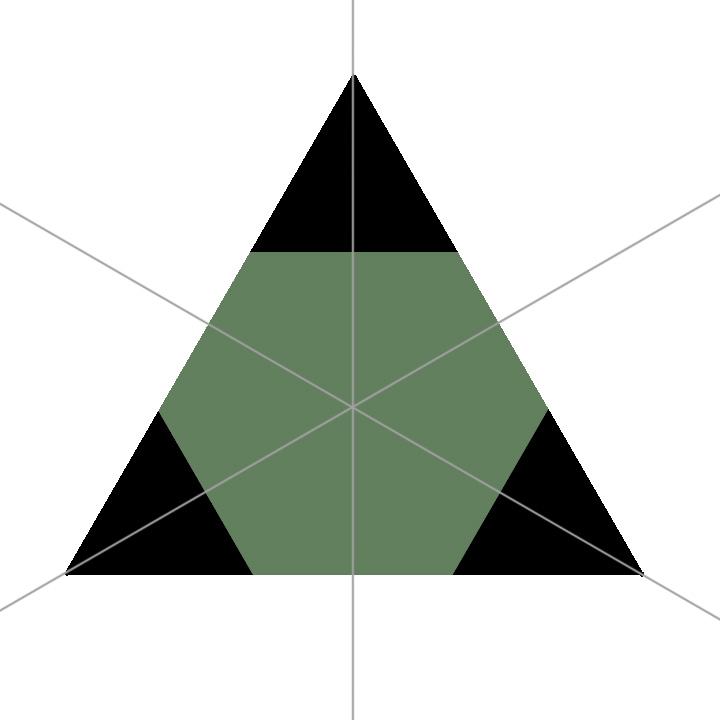
\includegraphics[width=2cm]{newtriangle_copya}\\\hline
			3 & 9 & $\dfrac{1}{6}(x_1^9+2x_3^3+3x_1^1x_2^4)$ & 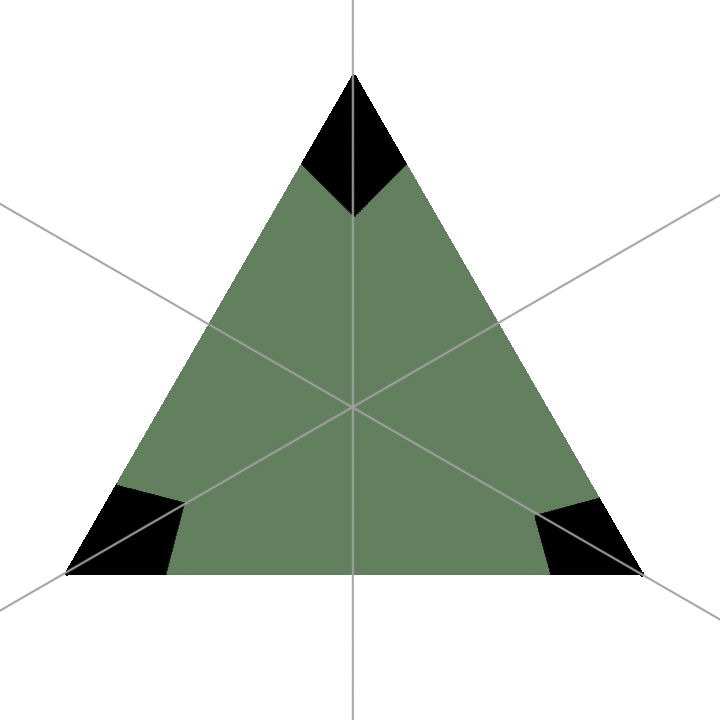
\includegraphics[width=2cm]{newtriangle_copy9}\\\hline
			4 & 12 & $\dfrac{1}{6}(x_1^{12}+2x_3^4+3x_1^2x_2^5)$ & 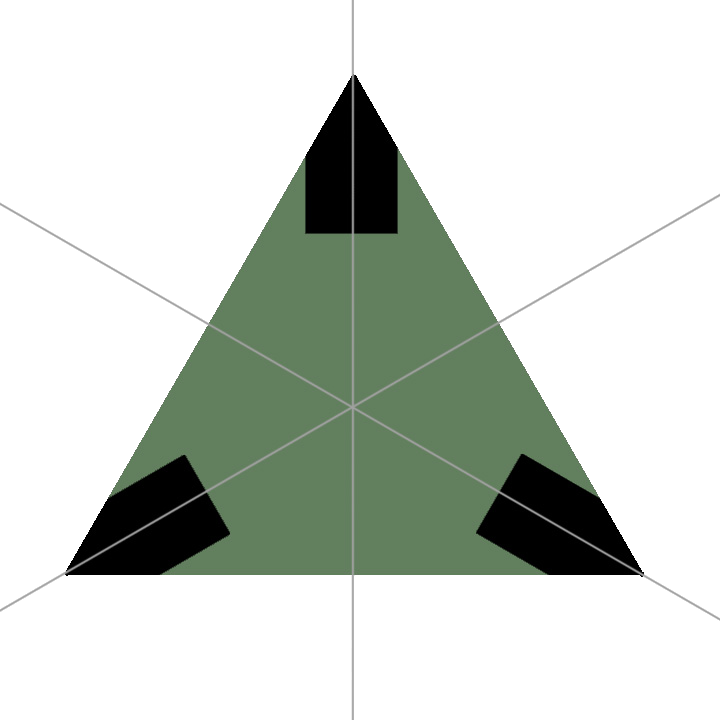
\includegraphics[width=2cm]{newtriangle_copy12}\\\hline
		\end{tabular}
	\end{table}
\end{frame}
%%%%%%%%%%%%%%%%%%%%%%%%%%%%%%%%%%%%%%%%%%%%%%%%%%%%%%%%%%
\begin{frame}{Understanding the Different Cases Concerning Flips}
	This is a hexagon inscribed inside a triangle:\\
		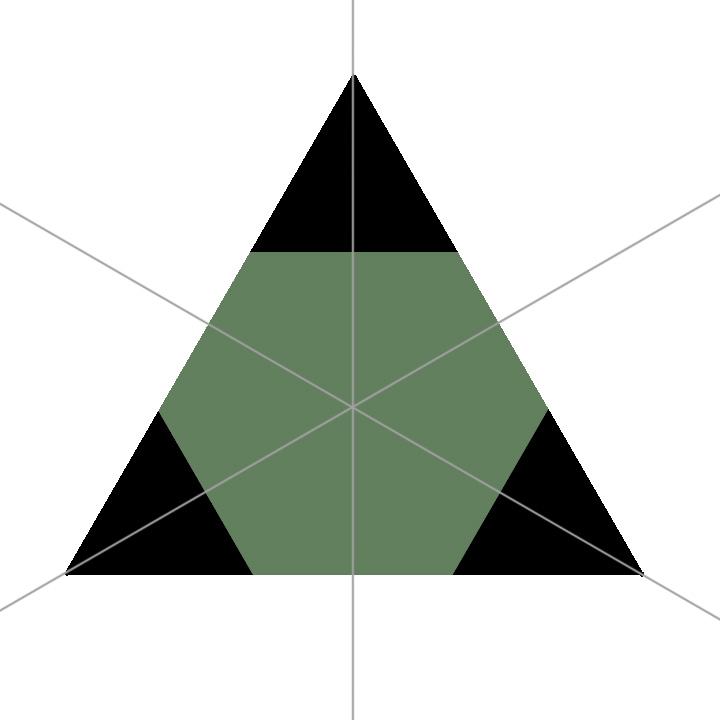
\includegraphics[width=3cm]{newtriangle_copya}
		$\dfrac{1}{6}(x_1^6+2x_3^2+3x_1^2x_2^2)$\\
	But so is this:\\
		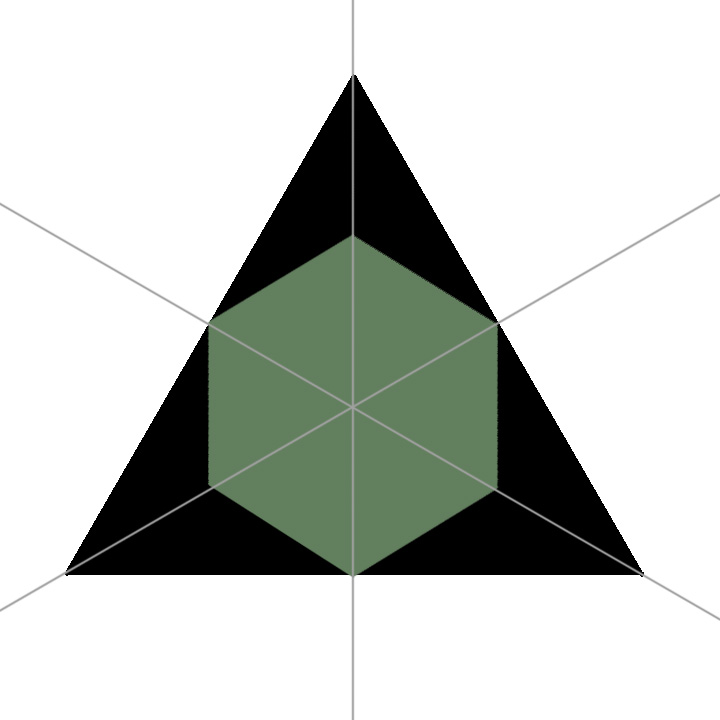
\includegraphics[width=3cm]{newtriangle_copy1}
		$\dfrac{1}{6}(x_1^6+2x_3^2+ 3x_2^3)$\\
\end{frame}
%%%%%%%%%%%%%%%%%%%%%%%%%%%%%%%%%%%%%%%%
\begin{frame}
	Thankfully we are able to draw the second picture another way.
	\begin{center}
		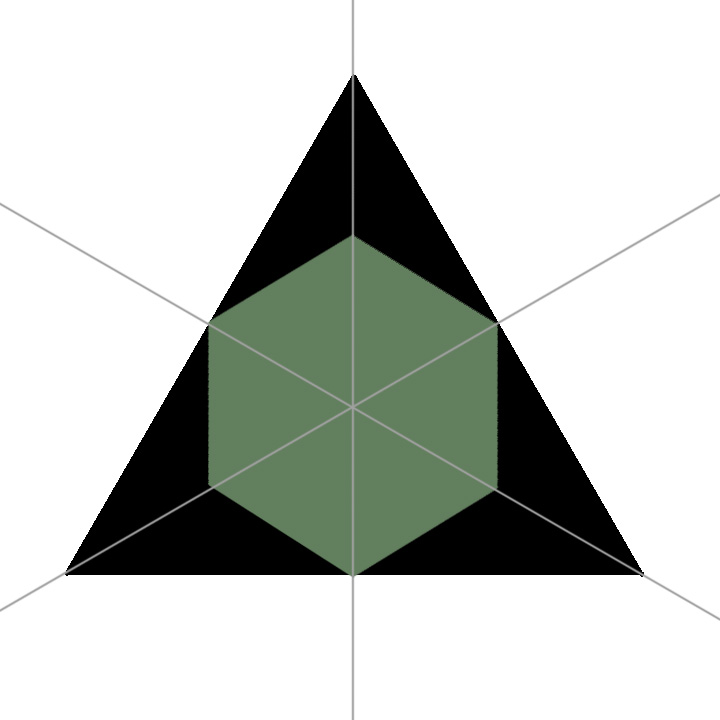
\includegraphics[width=3cm]{newtriangle_copy1}
		\mapsto
		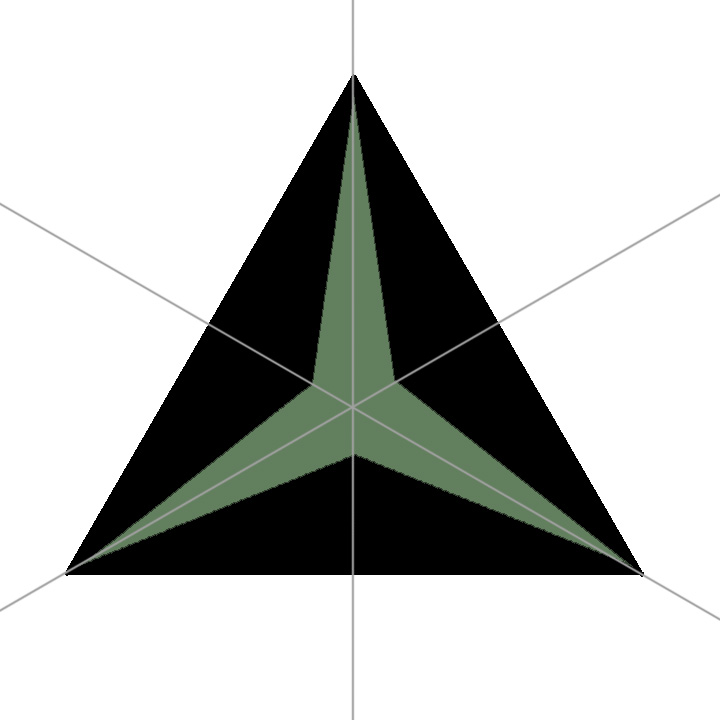
\includegraphics[width=3cm]{newtriangle_copyb}
	\end{center}
	Both of these shapes have the same cycle index.\\
  \end{frame}
  %%%%%%%%%%%%%%%%%%%%%%%%%%%%%%%%%%%%%%%%%%%%%
  \begin{frame}{Embedding Matters}
	All together we now have two ways to construct $nk$-gons which are acted on by $D_k$ dihedral groups.\\
	\begin{itemize}
		\item Truncate vertices
		\item Subdivide edges
	\end{itemize}
\end{frame}
%%%%%%%%%%%%%%%%%%%%%%%%%%%%%%%%%%%%%%%%%%%%%
\begin{frame}
\begin{table}
\centering
\begin{tabular}{c|c|c|c}
n & nk& Truncated Vertices & Subdivision of Edges\\\hline
2 & 8 & 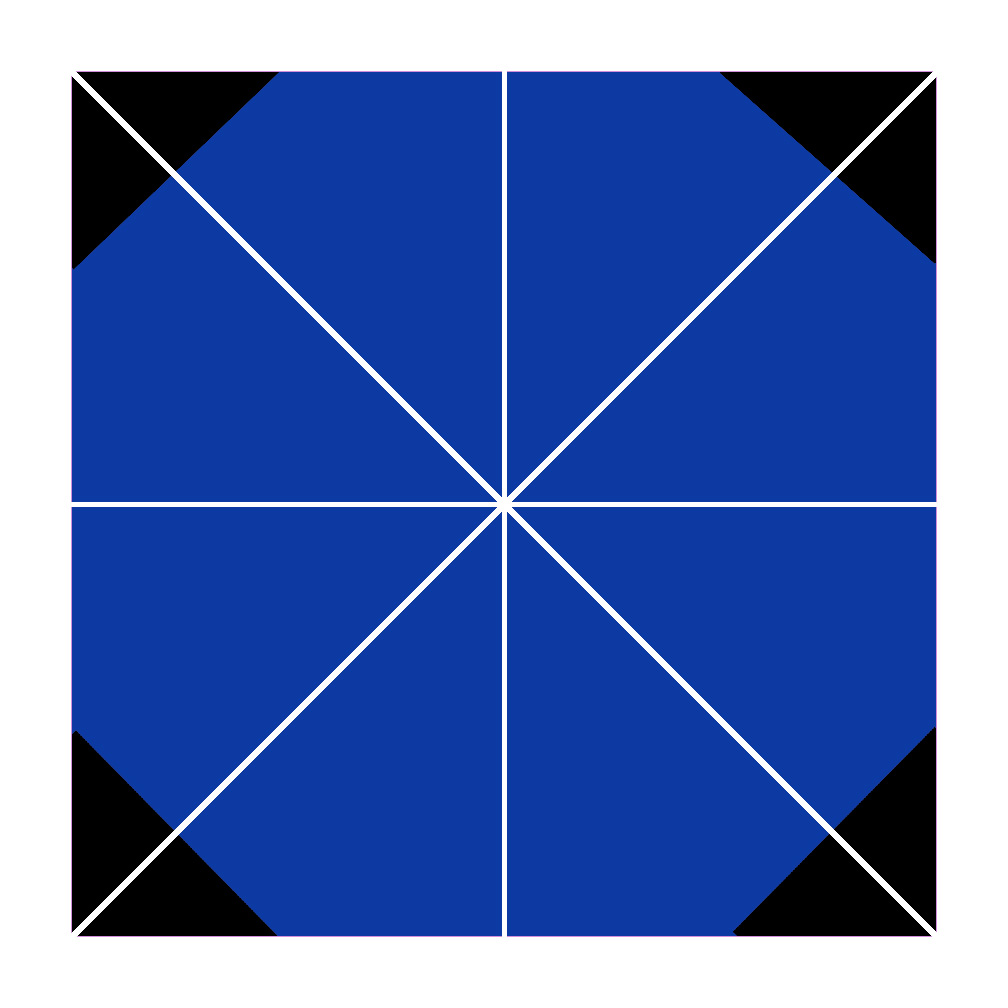
\includegraphics[width=3cm]{8tv}&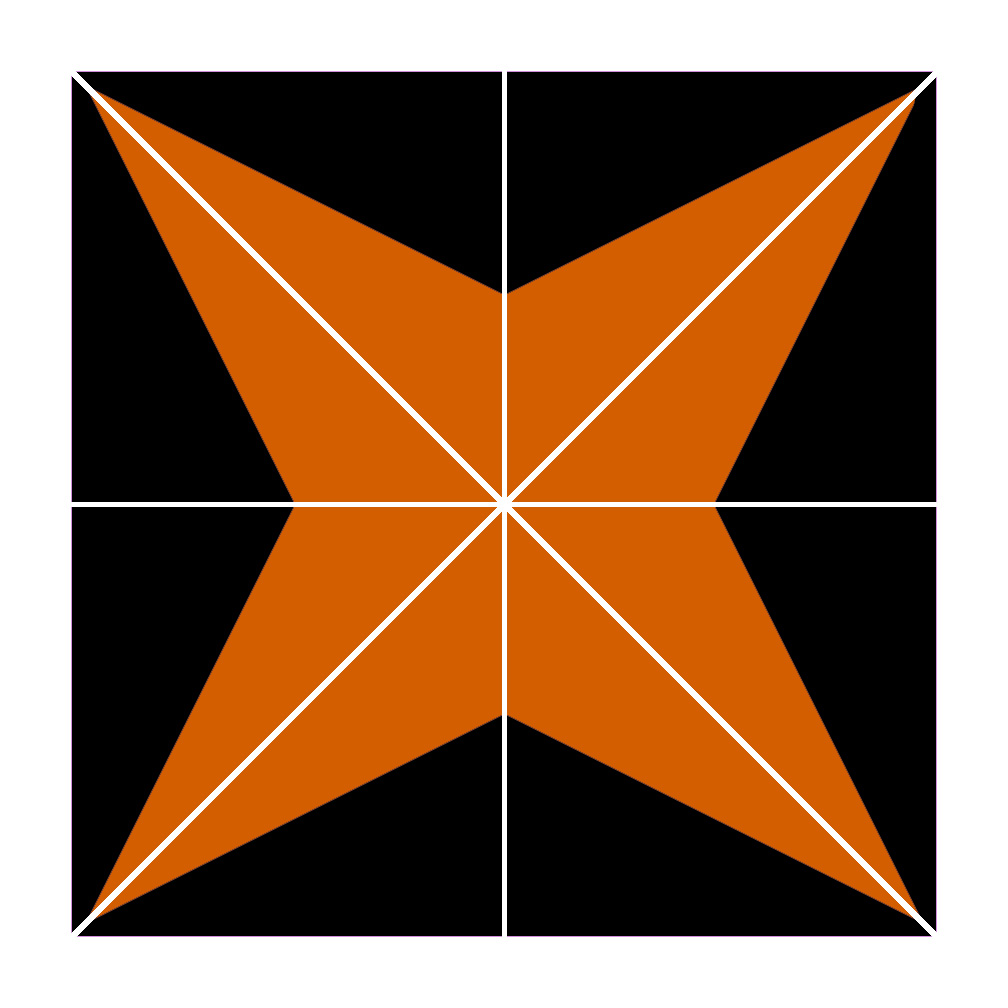
\includegraphics[width=3cm]{8se} \\\hline
3 & 12 & 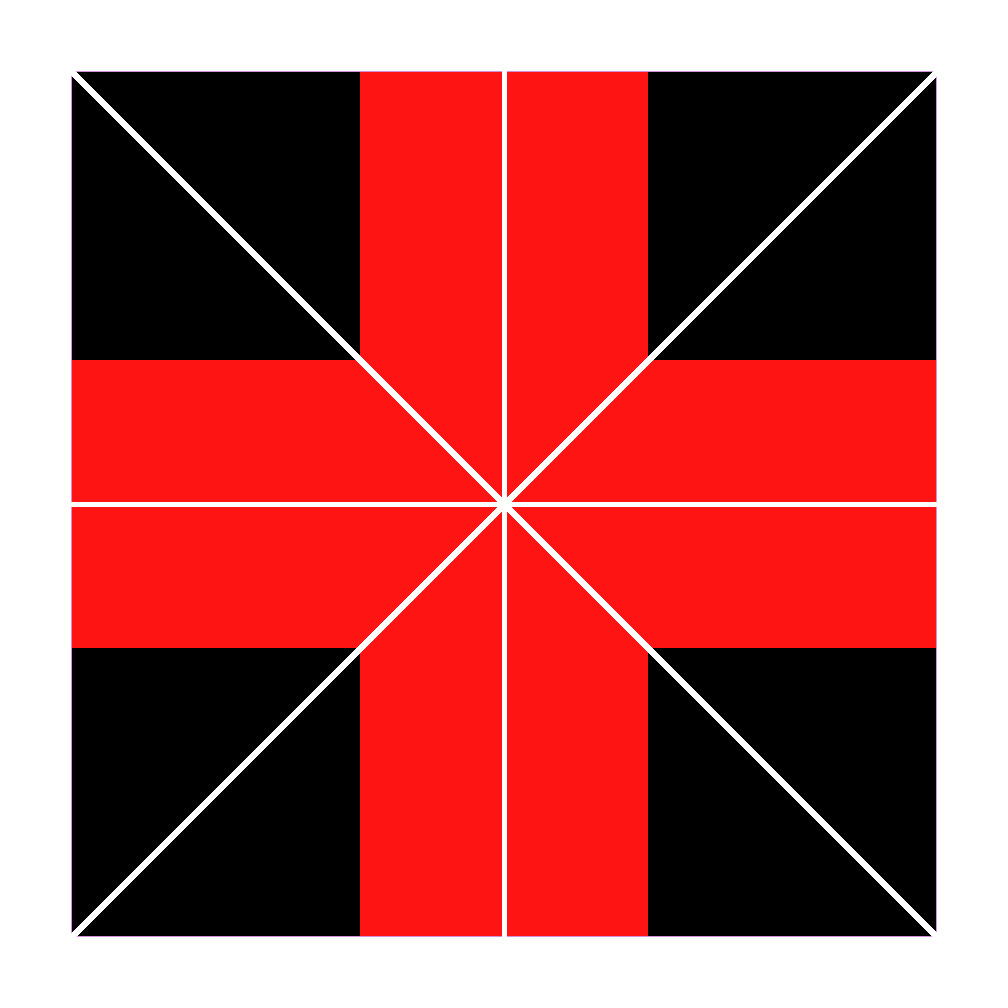
\includegraphics[width=3cm]{12tv} &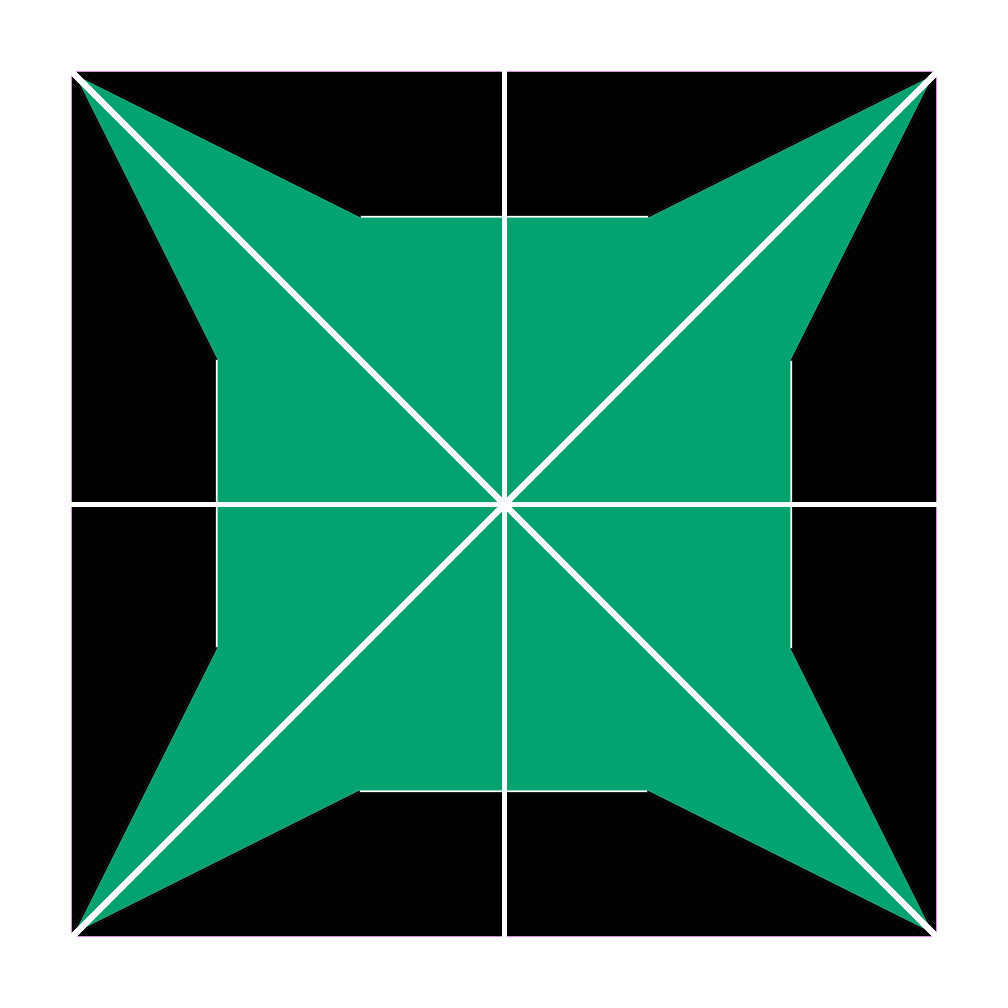
\includegraphics[width=3cm]{12se}\\\hline
\end{tabular}
\end{table}
\end{frame}
%%%%%%%%%%%%%%%%%%%%%%%%%%%%%%%%%%%%%%%%%%%%%%%%%%%%%%
\begin{frame}
\begin{table}
\centering
\begin{tabular}{c|c|c|c}
n & nk & Truncated Vertices & Subdivision of Edges \\\hline
5 & 20 & 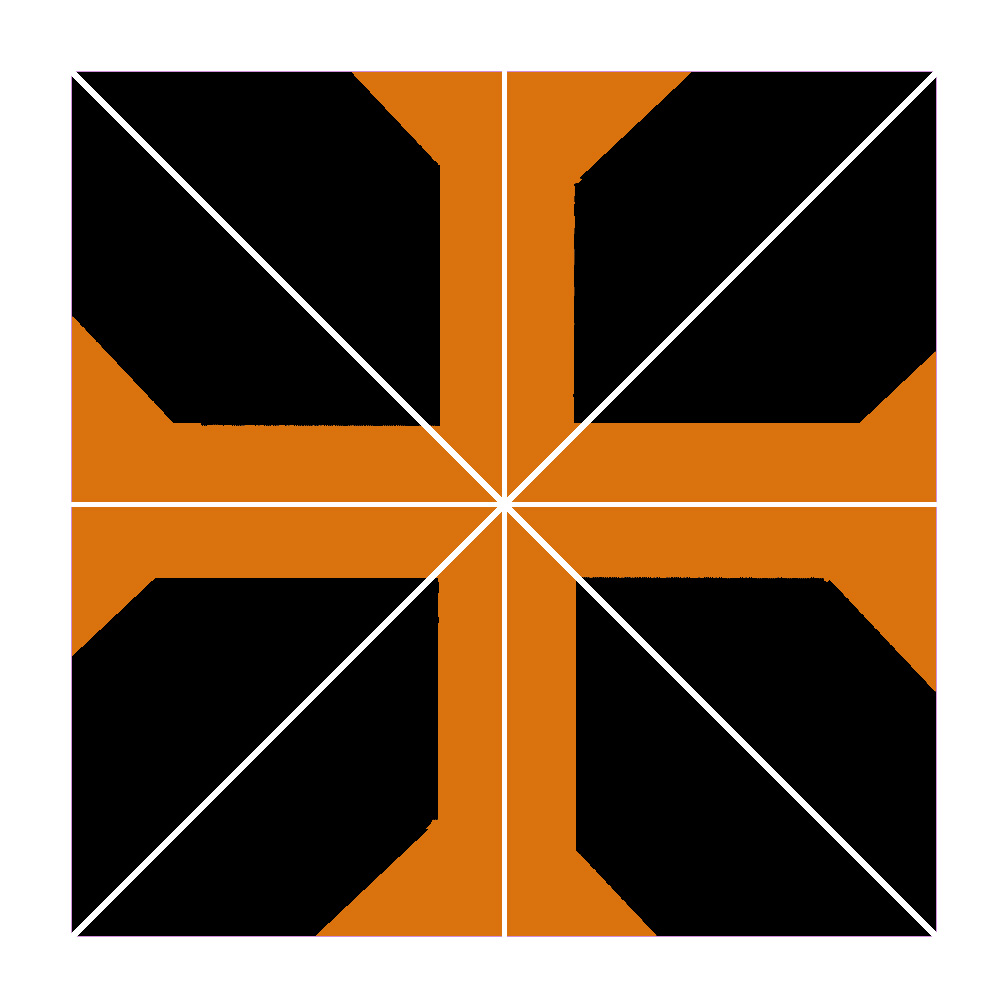
\includegraphics[width=3cm]{20tv} &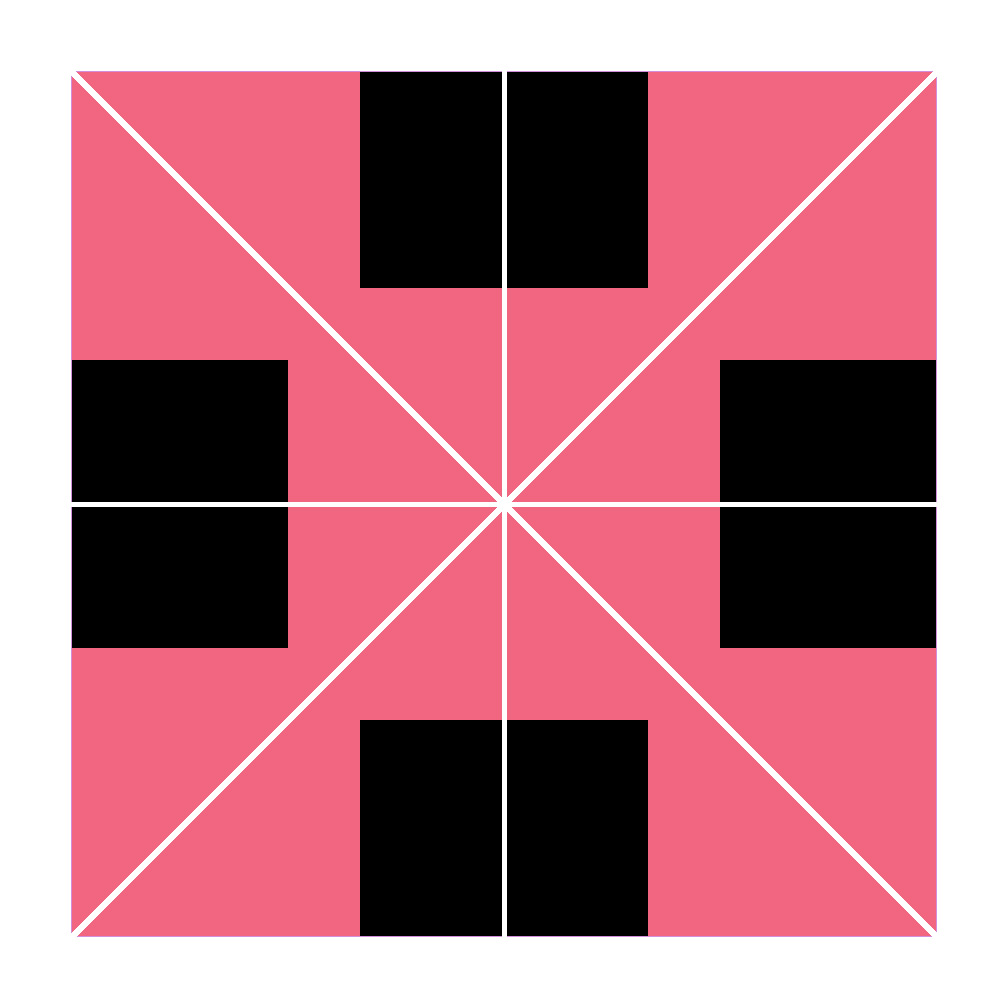
\includegraphics[width=3cm]{20se} \\\hline
6 & 24 & 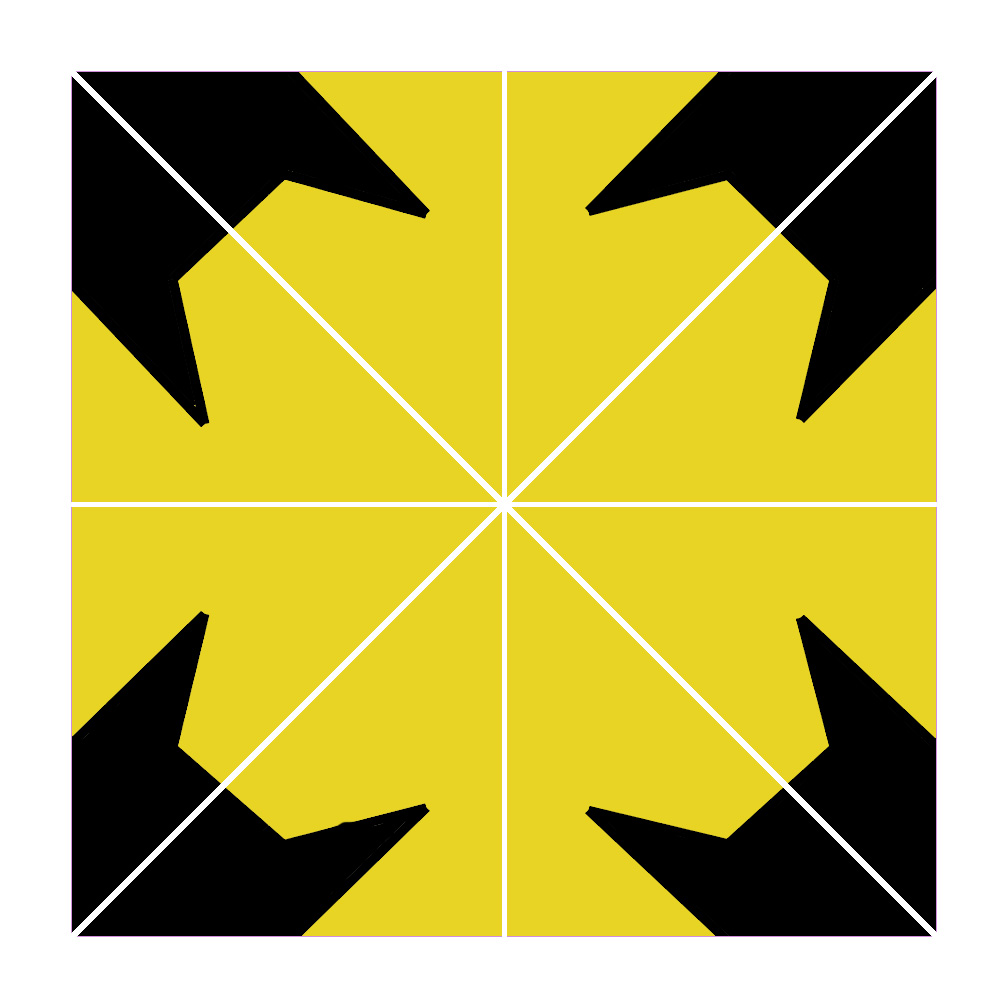
\includegraphics[width=3cm]{24_tv} &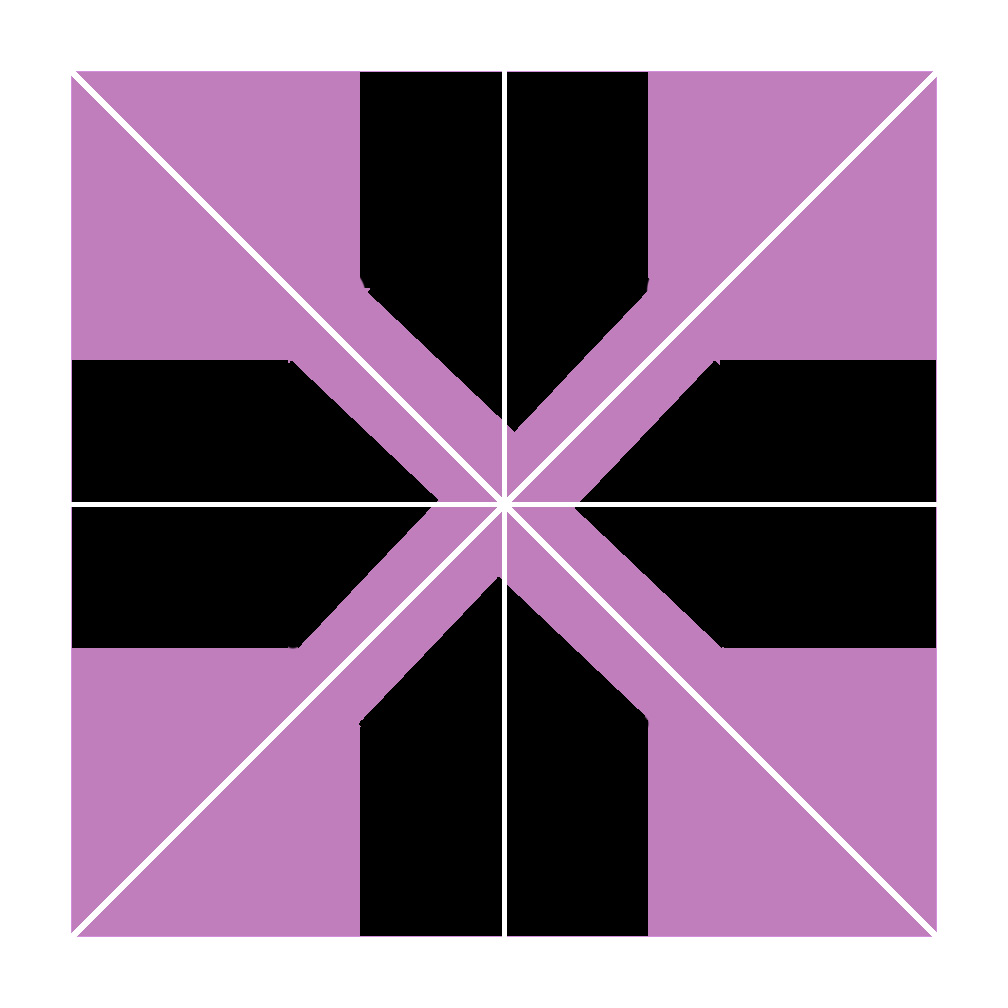
\includegraphics[width=3cm]{24se}\\\hline
\end{tabular}
\end{table}
\end{frame}
%%%%%%%%%%%%%%%%%%%%%%%%%%%%%%%%%%%%%%%%%%%%%%%%%%%%%
\begin{frame}
	Cycle index of a triangle:
	$x_1^3+2x_3^1+3x_1^1 x_2^1$\\

	\begin{table}
		\centering
		\begin{tabular}{l|c|l}
			n &
            Truncated Vertices &
            Subdivision of Edges\\ \hline
			2 &
            $\frac{1}{6}$($x_1^6+2x_3^2+$\colorbox{yellow}{$3x_1^2x_2^2$}) &
            $\frac{1}{6}$($x_1^6+2x_3^2+$ \colorbox{cyan}{$3x_2^3$})\\
			3 &
            $\frac{1}{6}$($x_1^9+2x_3^3+$\colorbox{pink}{$3x_1^1x_2^4$})  &
            $\frac{1}{6}$($x_1^9+2x_3^3+$\colorbox{pink}{$3x_1^1x_2^4$})\\
			4 &
            $\frac{1}{6}$($x_1^{12}+2x_3^4+$\colorbox{yellow}{$3x_1^2x_2^5$}) &
            $\frac{1}{6}$($x_1^{12}+2x_3^4+$\colorbox{cyan}{$3x_2^6$})\\
			5&
            $\frac{1}{6}$($x_1^{15}+2x_3^5+$\colorbox{pink}{$3x_1^1x_2^7$}) &
			$\frac{1}{6}$($x_1^{15}+2x_3^5+$\colorbox{pink}{$3x_1^1x_2^7$})\\
		\end{tabular}
		\caption{$D_3 \circlearrowright 3n$-gon}
	\end{table}
\end{frame}
%%%%%%%%%%%%%%%%%%%%%%%%%%%%%%%%%%%%%%%%%%%%%%%%%%%%%%%%%%%%%%%%%%%%%%%%%%
\begin{frame}{The Pattern:$D_3 \circlearrowright$ $n3$-gon}
\[\dfrac{1}{6}\Bigg(x_1^{3n}+(3-1)x_3^n +
\begin{cases}
3x_1^1x_2^{(3n-1)/2} & \text{n odd, V-E flip} \\
3x_1^2x_2^{(3n-2)/2} & \text{n even, E-E flip}\\
3x_1^2x_2^{(3n)/2} & \text{n even, V-V flip}
\end{cases}\Bigg)\]
 \end{frame}
%%%%%%%%%%%%%%%%%%%%%%%%%%%%%%%%%%%%%%%%%%%%%%%%%%%%%%%%%%%%%%%%%%%%%%%%%%%%%
 \begin{frame}{The Pattern:r $D_k \circlearrowright$ $nk$-gon with k-prime}
\[\dfrac{1}{2k}\Bigg(x_1^{kn}+(k-1)x_k^n +
\begin{cases}
kx_1^1x_2^{(kn-1)/2} & \text{n odd, V-E flip} \\
kx_1^2x_2^{(kn-2)/2} & \text{n even, E-E flip}\\
kx_1^2x_2^{(kn)/2} & \text{n even, V-V flip}
\end{cases}\bigg)\]
 \end{frame}
%%%%%%%%%%%%%%%%%%%%%%%%%%%%%%%%%%%%%%%%%%%%%%%%%%%%%%%%%%%%%%%%%%%%%%%%%%%%%%%%%
%\begin{frame}{Flips}
 %	Next, in order to find the polynomial of $d_k \circlearrowright nk-gon$ we need to add in the terms which 	  represent flips.\\
%	If $k$ is prime, then we have three cases:
%			\begin{enumerate}
%				\item $ kx_1^1x_2^{(kn-1)/2}$  for n odd $\longmapsto$\\
%				\item $kx_2^{(kn)/2}$ for n even$\longleftrightarrow$\\
%                \item $kx_1^2 x_2^{(kn-2)/2}$ for n even $|--|$\\
%			\end{enumerate}

%\end{frame}
\begin{frame}
Cycle index of a square:
$x_1^4+2x_4^1+x_2^2+x_1^2x_2^1+2x_2^2$\\

$D_4 \circlearrowright 4n$-gon\\

\begin{table}
\centering
\begin{tabular}{l|c|l}
n & Truncated Vertices & Subdivision of Edges\\ \hline
2 &
$\frac{1}{8}$($x_1^8+2x_4^2+x_2^4+$\colorbox{yellow}{$4x_1^2x_2^3$}) &
$\frac{1}{8}$($x_1^8+2x_4^2+x_2^4+$\colorbox{cyan}{$4x_2^4$})\\
3 &
$\frac{1}{8}$($x_1^{12} +2x_4^3+x_2^6+$ \colorbox{yellow}{$2x_1^2x_2^5$}$+$\colorbox{cyan}{$2x_2^6$}) &
$\frac{1}{8}$($x_1^{12} +2x_4^3+x_2^6+$ \colorbox{yellow}{$2x_1^2x_2^5$}$+$\colorbox{cyan}{$2x_2^6$})\\
4 &
$\frac{1}{8}$($x_1^{16}+2x_4^4+x_2^8+$\colorbox{yellow}{$4x_1^2x_2^7$}) &
$\frac{1}{8}$($x_1^{16}+2x_4^4+x_2^8+$\colorbox{cyan}{$4x_2^8$})\\
5 &
$\frac{1}{8}$($x_1^{20}+2x_4^5+x_2^{10}+$\colorbox{yellow}{$2x_1^2x_2^4$}$+$\colorbox{cyan}{$2x_2^{10}$}) &
$\frac{1}{8}$($x_1^{20}+2x_4^5+x_2^{10}+$\colorbox{yellow}{$2x_1^2x_2^4$}$+$\colorbox{cyan}{$2x_2^{10}$}\\
6 & $\dfrac{1}{8}$($x_1^{24}+2x_4^6+x_2^{12}+$\colorbox{yellow}{$4x_1^2x_2^{11}$}) & $\dfrac{1}{8}$($ x_1^24+2x_4^6+x_2^{12}+$ \colorbox{cyan}{$4x_2^{12}$})\\

\end{tabular}
\caption{$D_4 \circlearrowright 4n-gon$}
\end{table}
\end{frame}
%%%%%%%%%%%%%%%%%%%%%%%%%%%%%%%%%%%%%%%%%%%%%%
\begin{frame}{Algorithm for constructing the polynomials  which represent a dihedral group $D_k$ acting on a $nk-gon$.}
So for any $D_n$ acting on a $nk-gon$ we can produce the flips using cases:\\
	 $k$ Even:\\
			\begin{itemize}
    			\item $k/2x_1^2x_2^{(kn-2)/2}+k/2x_2^{kn/2}$ n odd ( V-V flips + E-E flips)
                \item $kx_1^2x_2^{(kn-2)/2}$ n even (E-E flips)
                \item $kx_2^{kn/2}$ n odd (V-V flips)
             \end{itemize}
         $k$ Odd:\\
         	\begin{itemize}
            	\item $kx_1^1x_2^{nk/2}$ n odd (V-E flips)
                \item $kx_2^{nk/2}$ n even (E-E flips)
                \item $kx_1^2x_2^{(nk-2)/2}$ n even (V-V flips)
            \end{itemize}

\end{frame}
%%%%%%%%%%%%%%%%%%%%%%%%%%%%%%%%%%%%%%%%%%%%%%%%%%%%%%%%%%%%
\begin{frame}
\begin{table}
\centering
\begin{tabular}{c|c|c|c|c|c|c}
1&
$x_1^1$ &&&&&
\\\hline
&$e$ &&&&&
\\\hline
2&
$x_1^2$ &
\textcolor{orange}{$x_2^1$} &&
\\\hline
& $e$ &&
\textcolor{orange}{180 \textdegree} &&&
\\\hline
3 &
$x_1^3$ &&
\textcolor{green}{$x_3^1$}&&&
\\\hline
& $e$ &&
\textcolor{green}{120\textdegree, 240\textdegree}&&
\\\hline
4 &
$x_1^4$ &
\textcolor{orange}{$x_2^2$} &&
\textcolor{purple}{$x_4^1$} &
\\\hline
& $e$ &
\textcolor{orange}{180 \textdegree} &&
\textcolor{purple}{90 \textdegree, 270\textdegree}&&
\\\hline
6&
$x_1^6$ &
\textcolor{orange}{$x_2^3$} &
\textcolor{green}{$x_3^2$} &&
\textcolor{blue}{$x_6^1$}&
\\\hline
\end{tabular}
\end{table}
\end{frame}


%%%%%%%%%%%%%%%%%%%%%%%%%%%%%%%%%%%%%%%%%%%%%%%%%%%%%%%%%%%%%
% \begin{frame}
% \begin{table}
% \centering
% \begin{tabular}{c|c|c|c|c|c|c|c|c|c}
% 1 & $x_1^1$ &\\\hline

% & ID&\\\hline

% 2 & $x_1^2$ & \textcolor{orange}{$x_2^1$} &\\\hline

% & ID & \textcolor{orange}{180 \textdegree} &\\\hline

% 3& $x_1^3$ & \textcolor{green}{$2x_3^1$} &\\\hline

% & ID & \textcolor{green}{120\textdegree, 240\textdegree}  \\\hline

% 4& $x_1^4$ & \textcolor{orange}{$x_2^2$} & \textcolor{red}{$2x_4^1$}\\\hline

% & ID & \textcolor{orange}{180 \textdegree} & \textcolor{red}{90 \textdegree, 270\textdegree}

% 6 & $x_1^6$ & \textcolor{orange}{$x_2^3$} & \textcolor{green}{$2x_3^4$} & \textcolor{blue}{$x_6^1$}\\\hline

% & ID & \textcolor{orange}{180 \textdegree} & \textcolor{green}{120\textdegree, 240\textdegree} & \textcolor{red}{90 \textdegree, 270\textdegree} & \textcolor{blue}{60 \textdegree, 300 \textdegree}

% 12 & $x_1^{12}$ & \textcolor{orange}{$x_2^6$} & \textcolor{green}{$2x_3^4$} & \textcolor{red}{$2x_4^3$} & \textcolor{blue}{$2x_6^2$} & \textcolor{purple}{$4x_1^{12}$}\\\hline

% & ID & \textcolor{orange}{180 \textdegree} & \textcolor{green}{120\textdegree, 240\textdegree} & \textcolor{red}{90 \textdegree, 270\textdegree} & \textcolor{blue}{60 \textdegree, 300 \textdegree} & \textcolor{purple}{30\textdegree, 130\textdegree, 210\textdegree, 330\textdegree}
% \end{tabular}
% \end{table}
% \end{frame}
%%%%%%%%%%%%%%%%%%%%%%%%%%%%%%%%%%%%%%%%%%%%%%%%%%%%%%%%%%%%%%
\begin{frame}{Rotations for a k-gon}
	\begin{itemize}
		\item	Suppose $a_1,a_2,...,a_n$ are divisors of $k$.\\
 		\item For each divisor $a_i$ assemble the values which are coprime to it. \\
		\item Denote these coprime values $b_{ij}$ for each respective $a_i$.\\
		\item Now the \textbf{rotation} terms in our polynomial for the normal $k-gon$ will be:\\
		\begin{center}
        $\sum |b_{ij}|x^{k/a_i}_{a_i}$
        \end{center}
	\end{itemize}
\end{frame}
\begin{frame}{Rotations for $D_k \circlearrowright$ $nk$-gon}

\begin{center}
        $\sum |b_{ij}|x^{nk/a_i}_{a_i}$
        \end{center}
\end{frame}
%}}}

\end{document}
